{\bf 2026-10-08}\\

I have spent the better part of the last 10 days trying to figure out how to run a more realistic LAT toast sim. Here is what I have learned:
\begin{enumerate}
    \item A realistic SO TOAST sim is largely run through the use of the command line interface (CLI) from the sotodlib module (\verb+toast_so_sim+). The CLI has a huge (thousands) of possible command line arguments to specify which operators to apply and operator parameters. This interface can also likely take config files to ensure reproducibility but I haven't really played around with that.
    \item While adding the new pointing jitter operator to the list of possible operators to call in the CLI is fairly straightforward, it is not clear how/where to include calling the new operator in the pipeline of a toast sim.
    \item The large number of arguments are not really accompanied by clear instructions indicating which operators need to be specified for a particular type of simulation. For instance, I have been trying to scan a solar system object (SSO) for a semi-realistic simulation of a point-source. Turns out defining the SSO in your schedule does not make toast actually simulate the source, to do this, you need to enable the \verb+--sim_sso.enable+ argument. But this argument seems to also require other arguments to be specified. What those arguments are, and what they should be set to is not clear (for example, what beam file should I specify).
    \item Running from a CLI makes many interactive things like plotting the impact of my operator much more difficult.
\end{enumerate}

Before I can do anything, I need to make sure that running the toast sim CLI actually pull from my custom code (since my code is not yet incorporated into the greater TOAST, sotodlib packages). The instructions for doing this are mostly documented on the SO wiki page for using NERSC. In brief, the steps are:
\begin{enumerate}
    \item Create a custom conda environment.
    \item Install the sotodlib and toast packages from source.
\end{enumerate}

Once this is done, the new operator must be added to the list of available operators for \verb+toast_so_sim+



Because I did not want to deal with trying to figure out how to use the toast SSO method, I just had toast spit out the RA/Dec of where Mars was from its schedule, then adjusted my input maps to have a point source at that location. 

\begin{figure}[h!]
    \centering
    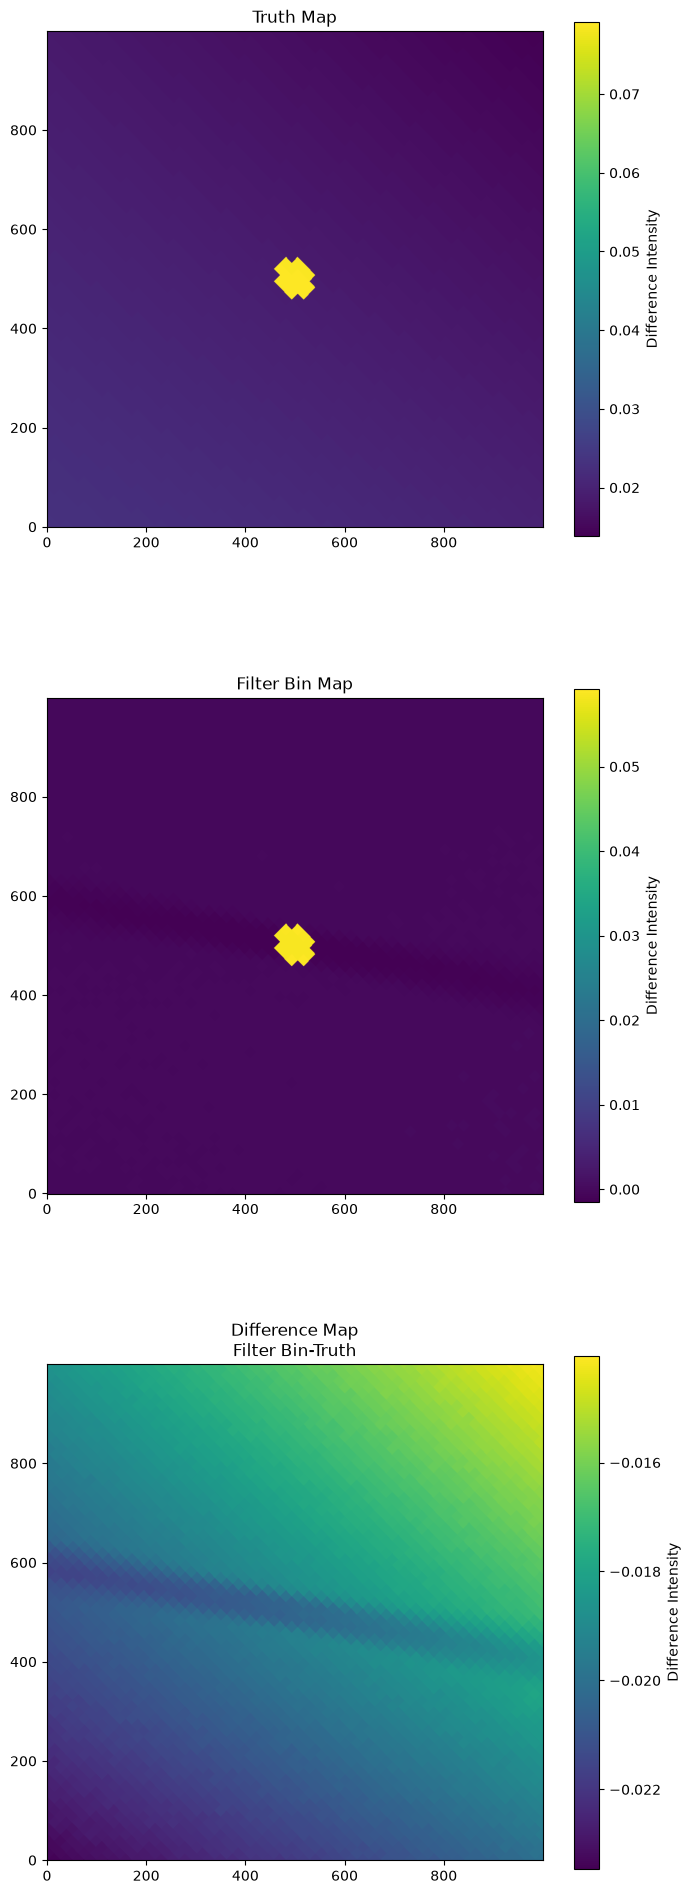
\includegraphics[width=0.5\textwidth]{Updates/figures/diff_map_2arcmin.png}
    \caption{Difference between input map and filter bin scan.}
    \label{fig:diff_map}
\end{figure}

To test that the CLI method was working, I ran a toast sim of my fake 'Mars' map without any pointing jitter. It took me a minute to get the inputs correct so that it would actually scan my custom map, and also run a filter bin mapmaker on the resulting TOD. After some trial and error, I was able to get the following map.